\section*{Test 9 Crowd of people leaving a large public space}

A public space with four exits and 1,000 persons equally distributed in the space. Choose a population of adult persons from Figure 5 with an immediate reaction and distribute the walking speeds over a population of 1,000 persons.
\vspace{4mm}

\noindent
\textbf{Step 1}: Record the time at which the last person leaves the space.

\vspace{4mm}

\noindent
\textbf{Step 2}: Door 1 and door 2 are locked and step 1 is repeated.

\vspace{4mm}

\noindent
The expected result is that it takes approximately twice as long to leave the space.



\begin{figure}[h]
	\centering
	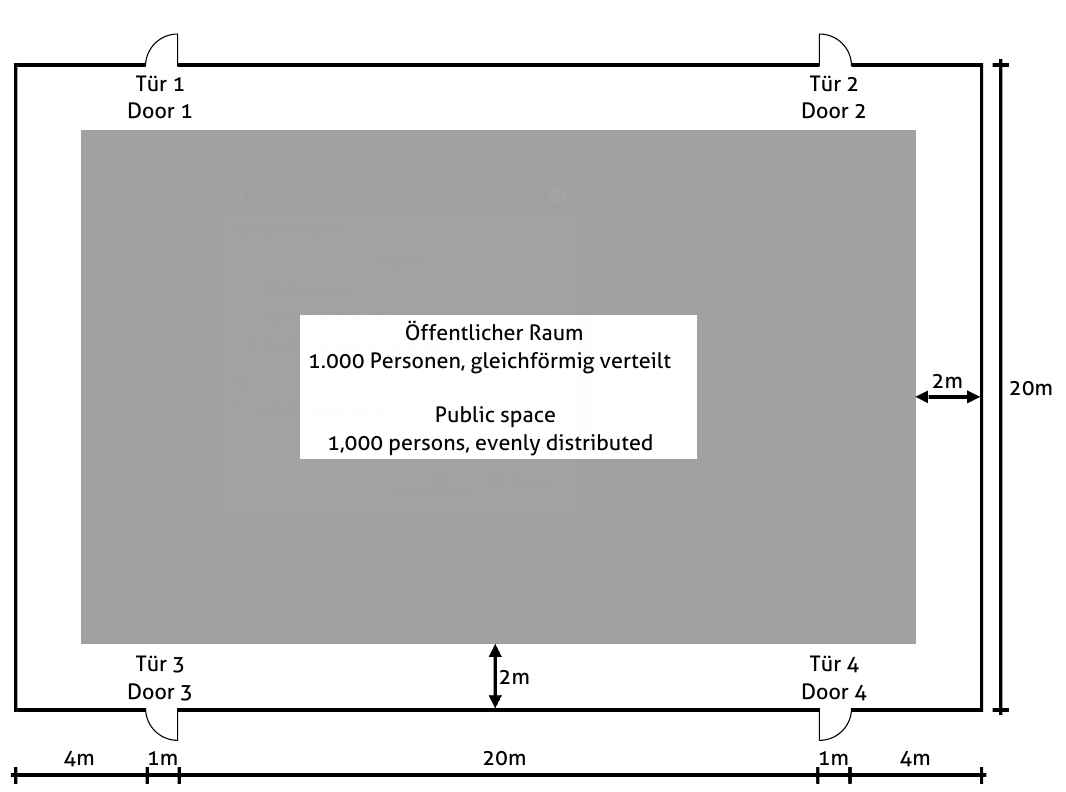
\includegraphics[scale=0.5]{test_description/Large_public_space_test_9.png}
	\caption{\footnotesize \textbf{Leaving a large public space}}
\end{figure}

